\subsection{Ionenbindung, kovalente Bindung und Metallbindung}
\label{subsec:ionenbindung-kovalente-bindung-metallbindung}

Valenzelektronen bestimmen, wie Atome miteinander wechselwirken. Aus ihrer
Abgabe, Aufnahme oder gemeinsamen Nutzung entstehen die wichtigsten Arten
chemischer Bindung\index{chemische Bindung}: die Ionenbindung\index{Ionenbindung},
die kovalente Bindung\index{kovalente Bindung} und die Metallbindung
\index{Metallbindung}.

Alle drei Bindungsarten beruhen auf demselben Grundgedanken: Die beteiligten
Atome erreichen durch eine veränderte Elektronenanordnung einen energetisch
günstigeren Zustand. Der Unterschied liegt darin, was mit den äußeren
Elektronen geschieht.
\FloatBarrier
\begin{figure}[H]
	\centering
	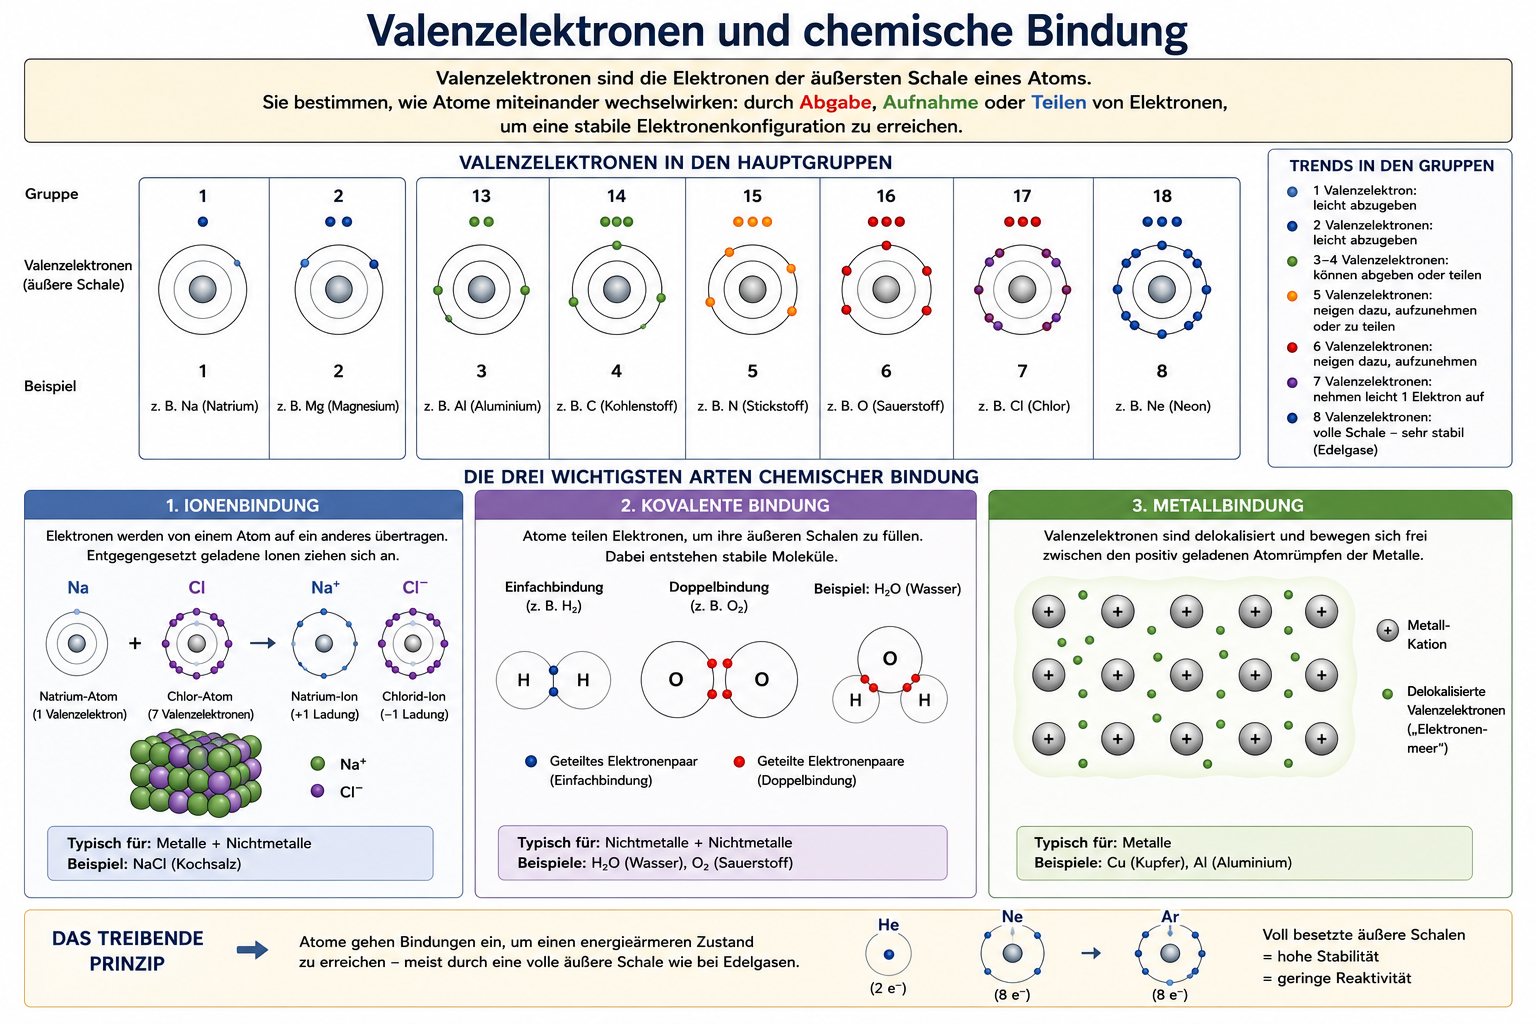
\includegraphics[width=\textwidth]{bilder/Valenzelektronen.png}
	\caption{Valenzelektronen und die wichtigsten Arten chemischer Bindung.
		Bei der Ionenbindung werden Elektronen übertragen. Bei der kovalenten Bindung
		teilen sich Atome Elektronenpaare. Bei der Metallbindung sind Valenzelektronen
		über viele Atomrümpfe hinweg delokalisiert.}
	\label{fig:valenzelektronen-bindungsarten}
\end{figure}

Bei der Ionenbindung wird ein oder werden mehrere Elektronen von einem Atom
auf ein anderes übertragen. Ein Atom gibt Elektronen ab und wird dadurch
positiv geladen. Das andere Atom nimmt Elektronen auf und wird dadurch negativ
geladen. Es entstehen Ionen\index{Ion}, also elektrisch geladene Atome oder
Atomgruppen.

Ein typisches Beispiel ist Natriumchlorid\index{Natriumchlorid}. Natrium besitzt
ein äußeres Elektron, das es leicht abgeben kann. Chlor besitzt sieben
Valenzelektronen; zur vollständig besetzten äußeren Schale fehlt ihm nur ein
Elektron. Überträgt Natrium sein äußeres Elektron auf Chlor, entstehen ein
positiv geladenes Natriumion und ein negativ geladenes Chloridion. Die
entgegengesetzten Ladungen ziehen sich an und bilden ein Ionengitter.

Bei der kovalenten Bindung werden Elektronen nicht vollständig übertragen,
sondern von zwei Atomen gemeinsam genutzt. Man spricht daher auch von einer
Elektronenpaarbindung\index{Elektronenpaarbindung}. Diese Bindungsart tritt
besonders häufig zwischen Nichtmetallen auf.

Ein einfaches Beispiel ist das Wasserstoffmolekül \( \mathrm{H_2} \). Jedes
Wasserstoffatom besitzt ein Elektron. Beide Atome teilen sich ein gemeinsames
Elektronenpaar. Dadurch erreicht jedes Wasserstoffatom näherungsweise die
stabile Zweierkonfiguration, wie sie beim Helium vorliegt.

Auch das Wassermolekül \( \mathrm{H_2O} \) lässt sich auf diese Weise
anschaulich verstehen. Sauerstoff besitzt sechs Valenzelektronen und teilt
jeweils ein Elektronenpaar mit zwei Wasserstoffatomen. Dadurch entstehen zwei
kovalente Bindungen.

Bei der Metallbindung ist die Situation anders. Metalle besitzen
Valenzelektronen, die nicht fest zu einem einzelnen Atom gehören. Stattdessen
sind sie über viele Atomrümpfe hinweg delokalisiert. Man kann sich ein Metall
anschaulich als ein Gitter positiv geladener Atomrümpfe vorstellen, zwischen
denen sich bewegliche Elektronen befinden.

Diese frei beweglichen Elektronen erklären viele typische Eigenschaften von
Metallen: elektrische Leitfähigkeit, Wärmeleitfähigkeit, metallischen Glanz und
Verformbarkeit. Besonders wichtig ist dabei, dass Elektronen im Metall nicht
nur lokale Bindungen zwischen zwei Atomen bilden, sondern sich über den
gesamten Festkörper ausbreiten können.

\begin{PhysicsBox}[Drei Bindungsarten aus Sicht der Elektronen]
	\label{box:drei-bindungsarten-elektronen}
	Die wichtigsten chemischen Bindungsarten unterscheiden sich durch das Verhalten
	der Valenzelektronen:
	
	\begin{itemize}
		\item \textbf{Ionenbindung:} Elektronen werden von einem Atom auf ein anderes
		übertragen.
		\item \textbf{Kovalente Bindung:} Atome teilen sich Elektronenpaare.
		\item \textbf{Metallbindung:} Valenzelektronen sind über viele Atomrümpfe
		hinweg delokalisiert.
	\end{itemize}
	
	In allen Fällen bestimmen Elektronen die Struktur der Materie.
\end{PhysicsBox}

Diese drei Bindungsarten sind idealisierte Grundmodelle. In realen Stoffen
können Übergänge auftreten. Manche Bindungen sind weder rein ionisch noch rein
kovalent. Auch in Metallen und Halbleitern reicht ein einfaches Schalenbild
nicht mehr aus. Dort muss man die Elektronen zunehmend als Zustände in einem
größeren quantenmechanischen System betrachten.

Damit führt die chemische Bindung direkt zum nächsten Schritt: In Molekülen
und Festkörpern sind Elektronen nicht mehr nur einzelnen Atomen zugeordnet.
Ihre Verteilung im Raum wird entscheidend. Genau darum geht es im nächsten
Abschnitt über Molekülorbitale und Elektronendichte.